% Intended LaTeX compiler: xelatex
\documentclass[10pt, svgnames]{beamer}
\usepackage{graphicx}
\usepackage{longtable}
\usepackage{wrapfig}
\usepackage{rotating}
\usepackage[normalem]{ulem}
\usepackage{amsmath}
\usepackage{amssymb}
\usepackage{capt-of}
\usepackage{hyperref}
\usetheme{metropolis}
\author{Sappinandana Akamphon}
\date{\today}
\title{Design of Welded Joints}
\subtitle{ME 310: Mechanical Design}
\usepackage{booktabs}
\usepackage{pgfplots}
\usepackage{multirow}
\usepackage{smartdiagram}
\pgfplotsset{compat=1.18}
\definecolor{lightblue}{RGB}{180,220,255}
\institute{Department of Mechanical Engineering, TSE}
\date{}
\usetikzlibrary{patterns,shapes,arrows}
\AtBeginSection[]{\begin{frame}{Outline}\tableofcontents[currentsection]\end{frame}}
\hypersetup{
 pdfauthor={Sappinandana Akamphon},
 pdftitle={Design of Welded Joints},
 pdfkeywords={},
 pdfsubject={},
 pdfcreator={Emacs 30.0.50 (Org mode 9.6)}, 
 pdflang={English}}
\begin{document}

\maketitle

\section{Welding Types}
\label{sec:org57f72a8}
\begin{frame}[label={sec:org0789133}]{Shielded Metal Arc Welding}
\centering
\includegraphics[width=0.75\textwidth]{pictures/shield-metal-arc-welding} \\\empty
Electric arc to produce heat
\end{frame}

\begin{frame}[label={sec:orgca5166a}]{MIG Welding}
\centering
\includegraphics[width=0.5\textwidth]{pictures/gas-metal-arc-welding}
\begin{itemize}
\item uses consumable electrode
\item simple to learn
\item welds aluminum, nonferrous, and stainless steel
\item expensive
\item neat but difficult to troubleshoot
\end{itemize}
\end{frame}


\begin{frame}[label={sec:org8314e18}]{TIG welding}
\centering
\includegraphics[width=0.7\textwidth]{pictures/gas-tungsten-arc-welding}
\begin{itemize}
\item nonconsumable electrode
\item difficult to learn and troubleshoot
\item welds almost all materials
\item preferred welding in precision and fabrication industry
\end{itemize}
\end{frame}

\begin{frame}[label={sec:org8c442ab}]{Resistance Welding}
\begin{columns}
  \column{0.6\textwidth}
  \centering
  \includegraphics[width=0.9\textwidth]{pictures/resistance-spot-welding}
  \column{0.4\textwidth}
  \begin{itemize}
  \item uses Joules heating ($i^2R$) to generate heat
  \item often require large current (1000 - 100000 A)
  \item widespread use in automotive industry
  \end{itemize}
\end{columns}
\end{frame}

\begin{frame}[label={sec:org2056234}]{Gas Welding}
\centering
\includegraphics[width=0.5\textwidth]{pictures/gas-welding}
\begin{itemize}
\item uses combustion (Acetylene + $O_2$) to generate heat
\item slow but cheap
\item mainly for maintenance purposes.
\end{itemize}
\end{frame}

\section{Weld Geometry and Terminology}
\label{sec:org239928c}
\begin{frame}[label={sec:org2c0eb83}]{Weld type}
\begin{columns}
\begin{column}{0.7\columnwidth}
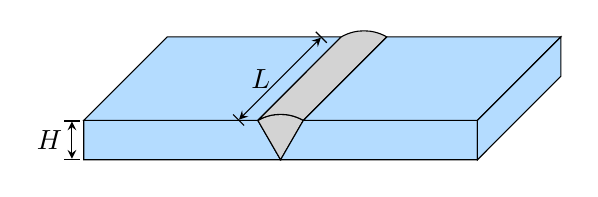
\begin{tikzpicture}[scale=0.5, >=stealth]
  \draw [fill=lightblue] (0,0) --++ (0:5) node(A){} --++ (120:1/cos{30}) node(B){} -- (0,1) -- cycle;
  \draw [fill=LightGrey] (A.center) -- (B.center) arc (120:60:1/cos{30}) node(C){} -- cycle;
  \draw [fill=lightblue] (10,0) node(E){} -- (A.center) -- (C.center) -- (10,1) node(F){} -- cycle;
  \draw [fill=lightblue] (0,1) --++ (45:3) --++ (0:4.42) node(D){} -- (B.center) -- cycle;
  \draw [fill=LightGrey] (B.center) -- (D.center) arc (120:60:1/cos{30}) -- (C.center) arc (60:120:1/cos{30});
  \draw [fill=lightblue, xshift=5.577cm] (0,1) --++ (45:3) --++ (0:4.42) node(G){} --++ (-135:3) -- cycle;
  \draw [fill=lightblue] (E.center) -- (F.center) -- (G.center) --++ (-90:1) -- cycle;
  % dimensioning
  \draw [|<->|] (0,0) ++ (180:0.3) --++ (90:1) node[midway, left]{$H$};
  \draw [|<->|] (B.center) ++ (180:0.5) --++ (45:3) node[midway, left]{$L$};
\end{tikzpicture}
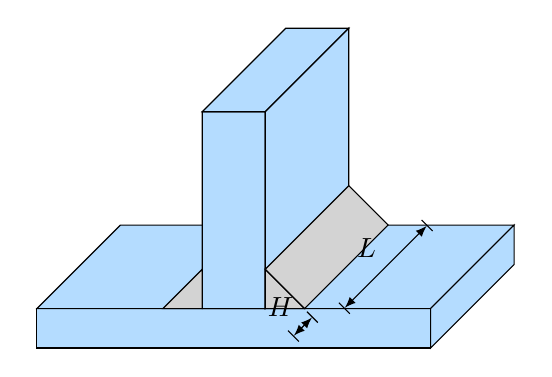
\begin{tikzpicture}[scale=0.5, >=latex]
  \draw [fill=lightblue] (0,0) --++ (0:10) --++ (90:1) node(B){} --++ (180:10) node(A){} node[midway, xshift=-0.4cm](D){} node[midway, xshift=0.4cm](E){} -- cycle;
  \draw [fill=lightblue] (A.center) --++ (45:3) --++ (0:10) node(C){} -- (B.center) -- cycle;
  \draw [fill=lightblue] (B.center) -- (C.center) --++ (-90:1) --++ (-135:3) -- cycle;
  \draw [fill=lightblue] (D.center) --++ (90:5) node(F){} --++ (0:1.6) node(G){} -- (E.center) --cycle;
  \draw [fill=lightblue] (F.center) --++ (45:3) --++ (0:1.6) -- (G.center) -- cycle;
  \draw [fill=lightblue] (E.center) -- (G.center) --++ (45:3) --++ (-90:5) -- cycle;
  \draw [fill=LightGrey] (D.center) --++ (90:1) --++ (-1,-1) -- cycle;
  \draw [fill=LightGrey] (E.center) --++ (90:1) node(H){} --++ (1,-1) node(I){} -- cycle;
  \draw [fill=LightGrey] (H.center) --++ (45:3) --++ (1,-1) -- (I.center) -- cycle;
  % dimensioning
  \draw [|<->|] (E.center) ++ (-45:1) --++ (45:0.707) node[midway, above left]{$H$};
  \draw [|<->|] (I.center) ++ (0:1) --++ (45:3) node[midway, above left]{$L$};
\end{tikzpicture}
\end{column}
\begin{column}{0.3\columnwidth}
\begin{itemize}
\item butt welds
\item fillet welds
\end{itemize}
\end{column}
\end{columns}
\end{frame}

\begin{frame}[label={sec:org2c2b5d5}]{Good Welds vs Bad Welds}
\begin{center}
\includegraphics[width=.9\linewidth]{./pictures/good-bead-vs-bad-bead.png}
\end{center}
\end{frame}

\section{Weld Stress Analysis}
\label{sec:orgb3b582b}
\begin{frame}[label={sec:org98c57bf}]{Welding Electrodes}
\centering 
\begin{tabular}{ p{3cm} p{2cm} p{2cm} p{2cm} }
  \toprule
  AWS Electrode Number & Tensile Strength (MPa) & Yield Strength (MPa) & Percent Elongation \\
  \midrule
  E60XX & 427 & 345 & 17-25 \\
  E70XX & 482 & 393 & 22 \\
  E80XX & 551 & 426 & 19 \\
  E90XX & 620 & 531 & 14-17 \\
  E100XX & 689 & 600 & 13-16 \\
  E120XX & 827 & 737 & 14 \\
  \bottomrule
\end{tabular}
\end{frame}

\begin{frame}[label={sec:orgf9099c2}]{Stress in Butt Welds}
\centering
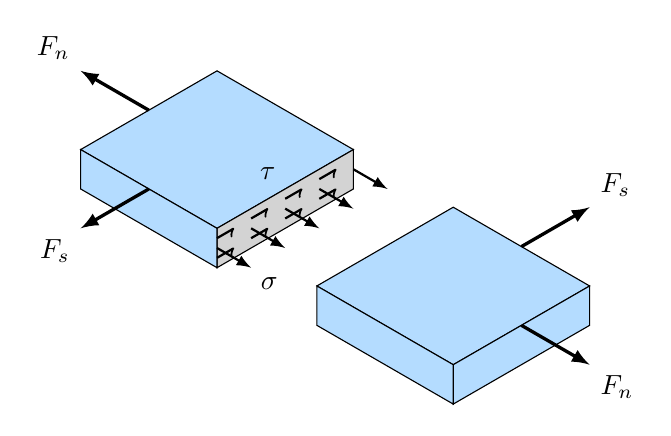
\begin{tikzpicture}[scale=1, >=latex]
  % top left piece
  \draw [fill=lightblue] (0,0) -- ++ (30:2) --++ (150:2) --++ (-150:2) node[midway](C){} --cycle node[midway](A){};
  \draw [fill=LightGrey] (0,0) -- ++ (30:2) --++ (-90:0.5) --++ (-150:2) --cycle;
  \draw [fill=lightblue] (0,0) -- ++ (150:2) --++ (-90:0.5) --++ (-30:2) --cycle;
  % bottom right piece
  \draw [fill=lightblue, xshift=3cm, yshift=-2*0.866cm] (0,0) -- ++ (30:2) node[midway](D){} --++ (150:2) node[midway](B){} --++ (-150:2) --cycle;
  \draw [fill=lightblue, xshift=3cm, yshift=-2*0.866cm] (0,0) -- ++ (30:2) --++ (-90:0.5) --++ (-150:2) --cycle;
  \draw [fill=lightblue, xshift=3cm, yshift=-2*0.866cm] (0,0) -- ++ (150:2) --++ (-90:0.5) --++ (-30:2) --cycle;
  % shear force pair
  \draw[->, very thick] (A.center) --++ (-150:1) node[below left]{$F_s$};
  \draw[->, very thick] (B.center) --++ (30:1) node[above right]{$F_s$};
  % normal force pair
  \draw[->, very thick] (C.center) --++ (150:1) node[above left]{$F_n$};
  \draw[->, very thick] (D.center) --++ (-30:1) node[below right]{$F_n$};
  % surface shear stress
  \foreach \x in {0,...,3} {
    \draw[-right to, thick] (0, -0.125) ++ (30:0.5*\x) --++ (30:0.25);
    \draw[-right to, thick] (0, -0.375) ++ (30:0.5*\x) --++ (30:0.25);
  }
  \draw (0,0) ++ (30:1) node[above left]{$\tau$};
  % surface normal stress
  \foreach \x in {0,...,4}
  \draw[->, thick] (0, -0.25) ++ (30:0.5*\x) --++ (-30:0.5);
  \draw (0,-0.25) ++ (-30:0.5) node[below right]{$\sigma$};
\end{tikzpicture}

\normalcolor
  \begin{align*}
    \sigma = \frac{F_n}{A_w} = \frac{F_n}{HL} \\
    \tau = \frac{F_s}{A_w} = \frac{F_s}{HL}
\end{align*}
\end{frame}


\begin{frame}[label={sec:org6839871}]{Stress in Fillet Welds}
\centering
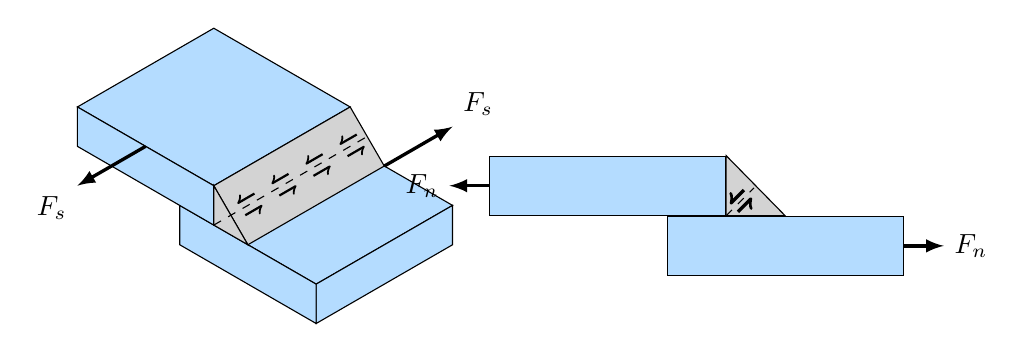
\begin{tikzpicture}[>=latex]
  % define nodes
  \path (0,0) ++ (-90:0.5) ++ (-30:0.5) node(E){} ++ (30:2) ++ (150:0.5) ++ (90:0.5) node(F){};
  % bottom right piece
  \draw [fill=lightblue, xshift=1.3cm, yshift=-1.25cm] (0,0) -- ++ (30:2) node[midway](D){} --++ (150:2) node[midway](B){} --++ (-150:2) --cycle;
  \draw [fill=lightblue, xshift=1.3cm, yshift=-1.25cm] (0,0) -- ++ (30:2) --++ (-90:0.5) --++ (-150:2) --cycle;
  \draw [fill=lightblue, xshift=1.3cm, yshift=-1.25cm] (0,0) -- ++ (150:2) --++ (-90:0.5) --++ (-30:2) --cycle;
  % top left piece
  \draw [fill=lightblue] (0,0) -- ++ (30:2cm) --++ (150:2cm) --++ (-150:2) node[midway](C){} --cycle node[midway](A){};
  %\draw [fill=LightGrey] (0,0) -- ++ (30:2) --++ (-90:0.5) --++ (-150:2) --cycle;
  \draw [fill=lightblue] (0,0) -- ++ (150:2) --++ (-90:0.5) --++ (-30:2) --cycle;
  % weld
  \draw [fill=LightGrey] (0,0) -- (E.center) node[midway](G){} --++ (30:2) -- (F.center) --cycle;
  \draw [fill=LightGrey] (0,0) --++ (-90:0.5) -- (E.center) --cycle;
  % shear force pair
  \draw[->, very thick] (A.center) --++ (-150:1) node[below left]{$F_s$};
  \draw[->, very thick] (B.center) --++ (30:1) node[above right]{$F_s$};
  % surface shear stress
  \draw[dashed] (0,0) ++ (-90:0.5) -- (G.center) --++ (30:2);
  \foreach \x in {0,...,3} {
    \draw[right to-, thick, xshift=0.3cm, yshift=-0.1cm] (0, -0.125) ++ (30:0.5*\x) --++ (30:0.25);
    \draw[-right to, thick, xshift=0.4cm] (0, -0.375) ++ (30:0.5*\x) --++ (30:0.25);
  }

  % Axial load in fillet weld
  \node at (5,0) [draw, rectangle, fill=lightblue, minimum height=0.75cm, minimum width=3cm, inner sep=0](M){};
  \node at (M.south east) [anchor=north west,draw, rectangle, fill=lightblue, minimum height=0.75cm, minimum width=3cm, xshift=-0.75cm](N){};
  % Weld
  \draw [fill=LightGrey](M.north east) -- (M.south east) --++ (0:0.75cm) --cycle;
  \draw [dashed] (M.south east) --++ (45:0.5);
  % Forces
  \draw [->, very thick] (M.west) --++ (180:0.5) node[left]{$F_n$};
  \draw [->, very thick] (N.east) --++ (0:0.5) node[right]{$F_n$};
  % Shear stresses
  \draw [right to-, very thick] (M.south east) ++ (0.05,0.15) -- ++ (45:0.25);
  \draw [-right to, very thick] (M.south east) ++ (0.15,0.05) -- ++ (45:0.25);
\end{tikzpicture}
\normalcolor

\begin{gather*}
  \tau = \frac{F_s}{HL} \\
  \tau = \frac{F_n}{HL}
\end{gather*}
\end{frame}


\begin{frame}[label={sec:orgd2d71cf}]{Stress in weld groups}
Assumptions

  \begin{itemize}
  \item parts being joined are rigid
  \item torsional and bending stresses can be found by

    \[\begin{gathered}
        \tau  = \frac{{Tr}}{{{J}}} \hfill \\
        \sigma  = \frac{{My}}{I} \hfill \\ 
      \end{gathered} \]
    
  \item must determine $I$ and $J$ of welds
  
\end{itemize}
\end{frame}

\begin{frame}[label={sec:org463adad}]{Finding \(I\) and \(J\) of welds}
\begin{itemize}
  \item Need to find center of rotation / neutral axis $\rightarrow$ weld center
\item Single weld -- centroid of weld cross-section
\item Multiple weld -- centroid of weld group
  \begin{align*}
    x_c = \frac{\int_A xdA}{A} = \frac{\sum x_{ci}A_i}{\sum A_i} \\
    y_c = \frac{\int_A ydA}{A} = \frac{\sum y_{ci}A_i}{\sum A_i}
  \end{align*}
\end{itemize}
\end{frame}

\begin{frame}[label={sec:orgc219c2b}]{Evaluating \(I\) and \(J\) for Individual Weld}
  \begin{itemize}
  \item for weld whose neutral axis passes through centroid / center of rotation coincides with centroid
    
  $$ I_c = \frac{L H^3}{12} $$
  $$ J_c = \frac{L H^3}{12} + \frac{H L^3}{12} $$

\item with multiple welds, neutral axis and/or center of rotation rarely coincides with individual centroids.
\end{itemize}
\end{frame}

\begin{frame}[label={sec:orge470511}]{Finding \(I\) and \(J\) for multiple welds}
\begin{itemize}
\item Once weld center is found, find $I$ and $J$ according to the center

  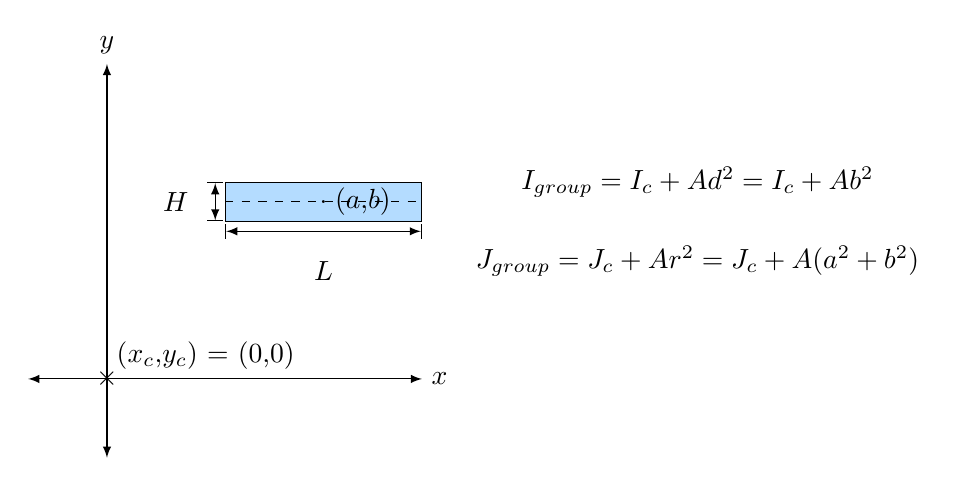
\begin{tikzpicture}[scale=0.5, >=latex]
    \draw[fill=lightblue] (3,4) rectangle ++(5,1) node[midway]{.} node[midway, xshift=0.5cm] {($a$,$b$)};
    \draw[dashed] (3,4.5) --++ (0:5);
    \draw[|<->|] (2.75,4) --++(90:1) node[midway,xshift=-0.5cm]{$H$};
    \draw[|<->|] (3, 3.75) --++ (0:5) node[midway,yshift=-0.5cm]{$L$};
    \draw (0,0) node{$\times$} node[above right]{($x_c$,$y_c$) = (0,0)};
    \draw[<->] (0,-2) --++(90:10) node[above]{$y$};
    \draw[<->] (-2,0) --++(0:10) node[right]{$x$};
    \draw[dashed] (0,0) --++ (0:5);
    \node at (15,5) {$I_{group} = I_c + A d^2 = I_{c} + Ab^{2}$ };
    \node at (15,3) {$J_{group} = J_c + A r^2 = J_{c} + A(a^{2}+b^{2})$};
  \end{tikzpicture}

\item Need to apply parallel axis theorem (if applicable)
\end{itemize}
\end{frame}

\begin{frame}[label={sec:org9dfebaa}]{Weld Joints under Torsion Example}
Determine the critical point in the welds and its state of stress. The weld throat thickness is 8 mm.

\begin{figure}[H]
  \centering
  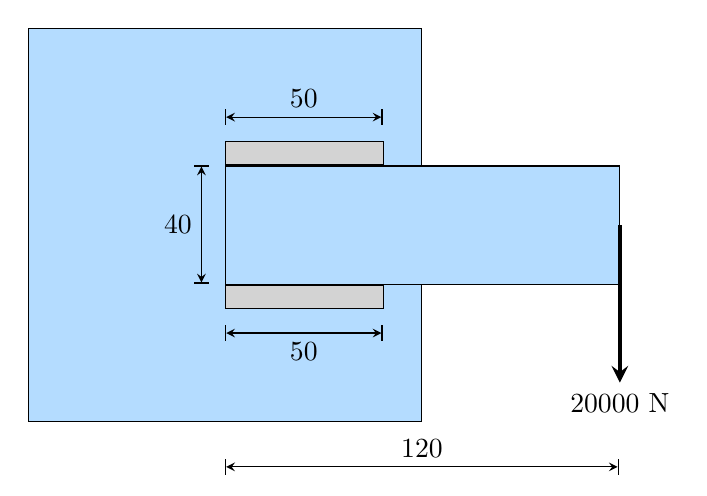
\begin{tikzpicture}[>=stealth]
    \node [draw, fill=lightblue, minimum height=5cm, minimum width=5cm](A){};
    \node at (A.east) [anchor=center, draw,  fill=lightblue, minimum height=1.5cm, minimum width=5cm](B){};
    \node at (B.north west) [anchor=south west, draw, fill=LightGrey, minimum height=0.3cm, minimum width=2cm](C){};
    \node at (B.south west) [anchor=north west, draw, fill=LightGrey, minimum height=0.3cm, minimum width=2cm](D){};
    % force
    \draw [->, ultra thick] (B.east) --++ (-90:2) node[below]{20000 N};
    % dimensions
    \draw [|<->|] (C.north west) ++ (90:0.3) --++ (0:2) node[midway, above]{50};
    \draw [|<->|] (D.south west) ++ (-90:0.3) --++ (0:2) node[midway, below]{50};
    \draw [|<->|] (C.south west) ++ (180:0.3) --++ (-90:1.5) node[midway, left]{40};
    \draw [|<->|] (D.south west) ++ (-90:2) --++ (0:5) node[midway, above]{120};
  \end{tikzpicture}
\end{figure}
\end{frame}

\begin{frame}[label={sec:org1b6cfa7}]{Break It Down}
\begin{itemize}
  \item Problem of shear loading + torsion
  \item Splitting the resultant stresses to analyze critical point
\end{itemize}
\end{frame}

\begin{frame}[label={sec:org2fb0475}]{Combination of Stresses}
\begin{figure}[H]
   \centering
   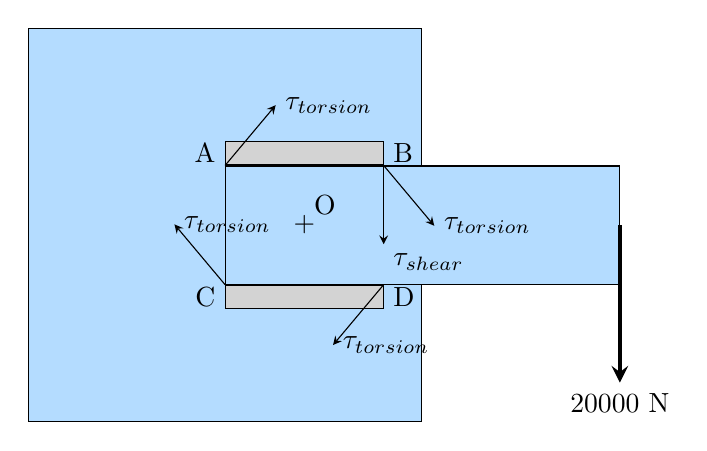
\begin{tikzpicture}[>=stealth]
     \node [draw, fill=lightblue, minimum height=5cm, minimum width=5cm](A){};
     \node at (A.east) [anchor=center, draw,  fill=lightblue, minimum height=1.5cm, minimum width=5cm](B){};
     \node at (B.north west) [anchor=south west, draw, fill=LightGrey, minimum height=0.3cm, minimum width=2cm](C){};
     \node at (B.south west) [anchor=north west, draw, fill=LightGrey, minimum height=0.3cm, minimum width=2cm](D){};
     \node at (C.west) [left]{A};
     \node at (C.east) [right]{B};
     \node at (D.west) [left]{C};
     \node at (D.east) [right]{D};
     \draw (C.south) ++ (-90:0.75) node{+} node[above right]{O};
     % force
     \draw [->, ultra thick] (B.east) --++ (-90:2) node[below]{20000 N};
     % stresses
     \draw [->] (C.south east) --++ (-90:1) node[below right]{$\tau_{shear}$};
     \draw [->] (C.south east) --++ (-50:1) node[right]{$\tau_{torsion}$};
     \draw [->] (D.north east) --++ (-130:1) node[right]{$\tau_{torsion}$};
     \draw [->] (D.north west) --++ (130:1) node[right]{$\tau_{torsion}$};
     \draw [->] (C.south west) --++ (50:1) node[right]{$\tau_{torsion}$};
   \end{tikzpicture}
 \end{figure}
\end{frame}

\begin{frame}[label={sec:org119a1e0}]{Shear Force}
\begin{align*}
  \tau_{shear} &= \frac{P}{2HL} = \frac{20000}{2(0.008)(0.05)} \\
               &= 25 \text{ MPa}
\end{align*}
\end{frame}

\begin{frame}[label={sec:org7b7e616}]{Torsion}
\begin{itemize}
\item Symmetric welds \(\rightarrow\) center of weld is at O

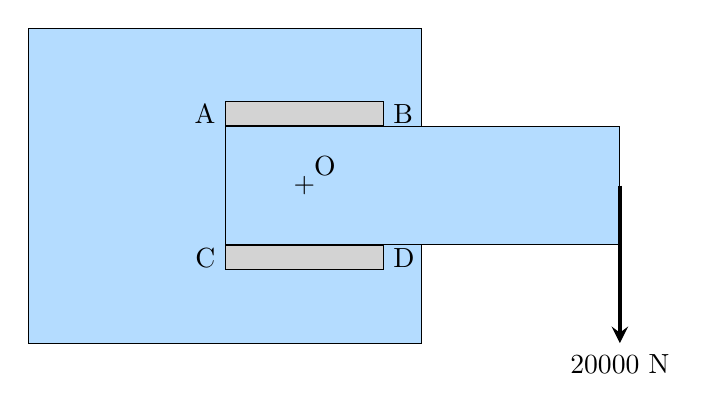
\begin{tikzpicture}[>=stealth]
  \node [draw, fill=lightblue, minimum height=4cm, minimum width=5cm](A){};
  \node at (A.east) [anchor=center, draw,  fill=lightblue, minimum height=1.5cm, minimum width=5cm](B){};
  \node at (B.north west) [anchor=south west, draw, fill=LightGrey, minimum height=0.3cm, minimum width=2cm](C){};
  \node at (B.south west) [anchor=north west, draw, fill=LightGrey, minimum height=0.3cm, minimum width=2cm](D){};
  \node at (C.west) [left]{A};
  \node at (C.east) [right]{B};
  \node at (D.west) [left]{C};
  \node at (D.east) [right]{D};
  \draw (C.south) ++ (-90:0.75) node{+} node[above right]{O};
  \draw [->, ultra thick] (B.east) --++ (-90:2) node[below]{20000 N};
\end{tikzpicture}

\begin{align*}
  \tau_{torsion} &= \frac{Tr}{J_{group}} = \frac{P L_o r_o}{J_{group}} \\
                 &= \frac{20000(0.12-0.05/2) r_o}{J_{group}}
\end{align*}
\end{itemize}
\end{frame}

\begin{frame}[label={sec:org89b470a}]{}
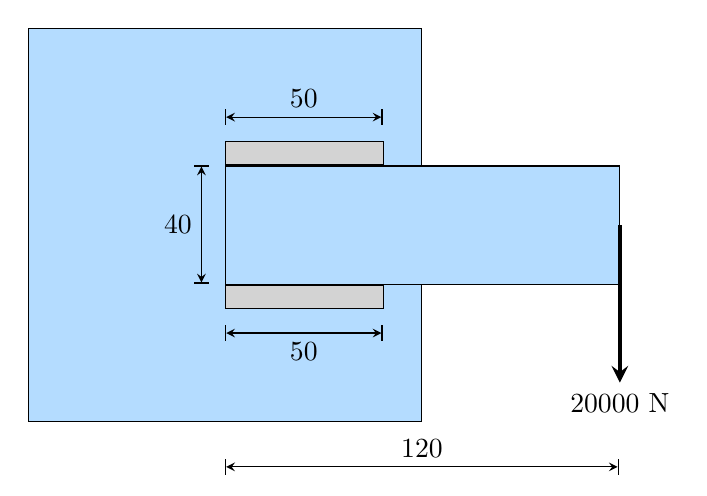
\begin{tikzpicture}[>=stealth]
  \node [draw, fill=lightblue, minimum height=5cm, minimum width=5cm](A){};
  \node at (A.east) [anchor=center, draw,  fill=lightblue, minimum height=1.5cm, minimum width=5cm](B){};
  \node at (B.north west) [anchor=south west, draw, fill=LightGrey, minimum height=0.3cm, minimum width=2cm](C){};
  \node at (B.south west) [anchor=north west, draw, fill=LightGrey, minimum height=0.3cm, minimum width=2cm](D){};
  % force
  \draw [->, ultra thick] (B.east) --++ (-90:2) node[below]{20000 N};
  % dimensions
  \draw [|<->|] (C.north west) ++ (90:0.3) --++ (0:2) node[midway, above]{50};
  \draw [|<->|] (D.south west) ++ (-90:0.3) --++ (0:2) node[midway, below]{50};
  \draw [|<->|] (C.south west) ++ (180:0.3) --++ (-90:1.5) node[midway, left]{40};
  \draw [|<->|] (D.south west) ++ (-90:2) --++ (0:5) node[midway, above]{120};
\end{tikzpicture}

\begin{align*}
  r_o &= \sqrt{ \left( \frac{L}{2} \right)^2 + d_o^2 } \\
  r_o &= \sqrt{ \left( \frac{0.05}{2} \right)^2 + 0.02^2 } \\
    &= 0.032 \text{ m}
\end{align*}
\end{frame}

\begin{frame}[label={sec:org038c58c}]{\(J_{c}\) of Welds}
\begin{align*}
  J_{group} &= J_c + A d_o^2 \\
            &= 2 \left[ \frac{HL^3}{12} +\frac{LH^3}{12} + LHd_o^2 \right] \\
            &= 2 \left[ \frac{(0.008)(0.05)^3}{12} + \frac{(0.05)(0.008)^3}{12} + (0.05)(0.008)(0.02)^2 \right] \\
            &= 1.70 \times 10^{-5} \text{ m}^4
\end{align*}
\end{frame}

\begin{frame}[label={sec:orgec17f80}]{Shear Stress from Torsion}
Now we have all the parameters we need, so we can substitute them back into the torsional shear stress equation, which gives

\begin{align*}
  \tau_{torsion} &= \frac{20000(0.12-0.05/2) r_o}{J_{group}} \\
                 &= \frac{20000(0.095)(0.032)}{1.7 \times 10^{-5}} \\
                 &= 3.58 \text{ MPa}
\end{align*}
\end{frame}

\begin{frame}[label={sec:org402b9da}]{Combining the Stress}
\begin{itemize}
  \item Combine using vector addition equation
\end{itemize}
\begin{align*}
  \left| \vec{\tau}_{torsion} + \vec{\tau}_{shear} \right|^2 &= \left| \vec{\tau}_{torsion} \right|^2 + \left| \vec{\tau}_{shear} \right|^2 + 2 \vec{\tau}_{torsion} \cdot \vec{\tau}_{shear} \\
                                                             &= \left| \vec{\tau}_{torsion} \right|^2 + \left| \vec{\tau}_{shear} \right|^2 + 2 \left| \vec{\tau}_{torsion} \right| \left| \vec{\tau}_{shear} \right| \cos \alpha
\end{align*}
\end{frame}

\begin{frame}[label={sec:orgab1c75a}]{Finding \(\alpha\)}
\begin{itemize}
  \item We don't really need $\alpha$, just $\cos \alpha$

\begin{align*}
  \cos \alpha &= \frac{L/2}{r_{O}} = \frac{L}{2r_{O}} \\
              &= \frac{0.05}{2(0.032)} = 0.78 \\
\end{align*}

  \item Substitute $\alpha$ into the vector addition formula to obtain the combined shear stress

\begin{align*}
  \left| \vec{\tau}_{torsion} + \vec{\tau}_{shear} \right|^2 &= 25^2 + 3.58^2 + 2(25)(3.58)(0.78) \\
                                                             &= 778 \\
  \left| \vec{\tau}_{torsion} + \vec{\tau}_{shear} \right| &= \left| \vec{\tau}_{total} \right| = 27.9 \text{ MPa}                                                        
\end{align*}
\end{itemize}
\end{frame}

\begin{frame}[label={sec:org26fc603}]{Stress in Weld joints under Bending}
 \centering
\includegraphics[scale=0.6]{pictures/dual-fillet-cantilever}
$$ \sigma = \frac{My}{I_{group}} $$
\end{frame}

\begin{frame}[label={sec:orgad358b6}]{Weld under Bending Example}
Determine the maximum load \(P\) that can be applied to the structure as shown below, given that the safety factor of the weld is 3. The weld has the effective throat thickness of 3 mm, and is made with E70XX series electrode.

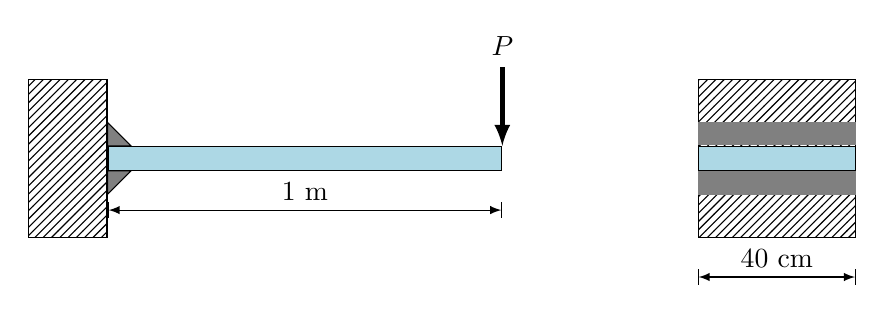
\begin{tikzpicture}[>=latex]
  \node at (0,0) [draw, rectangle, inner sep=0, fill=LightBlue, minimum height=0.3cm, minimum width=5cm](A){};
  \node at (A.west) [anchor=east, draw, pattern=north east lines, rectangle, minimum height=2cm, minimum width=1cm]{};
  \draw [fill=Grey](A.north west) --++ (90:0.3) -- ++(0.3, -0.3) -- cycle;
  \draw [fill=Grey](A.south west) --++ (-90:0.3) -- ++(0.3, 0.3) -- cycle;
  \draw [<-, ultra thick](A.north east) --++ (90:1) node[above]{$P$};
  \node at (A.south west)[yshift=-0.5cm](B){};
  \node at (A.south east)[yshift=-0.5cm](C){};
  \draw [|<->|] (B.center) -- (C.center) node[midway, above]{1 m};

  \node at (7,0) [anchor=east, draw, pattern=north east lines, rectangle, minimum height=2cm, minimum width=2cm](D){};
  \node at (D.center)[draw, rectangle, inner sep=0, fill=LightBlue, minimum height=0.3cm, minimum width=2cm](E){};
  \node at (E.north)[anchor=south, rectangle, inner sep=0, fill=Grey, minimum height=0.3cm, minimum width=2cm](){};
  \node at (E.south)[anchor=north, rectangle, inner sep=0, fill=Grey, minimum height=0.3cm, minimum width=2cm](){};

  \node at (D.south west)[yshift=-0.5cm](F){};
  \node at (D.south east)[yshift=-0.5cm](G){};
   \draw [|<->|] (F.center) -- (G.center) node[midway, above]{40 cm};
\end{tikzpicture}
\end{frame}


\begin{frame}[label={sec:org0e38177}]{Break It Down}
\begin{itemize}
  \item Shear force + bending
  \item Same stresses throughout
  \item From shear force
        \[\tau  = \frac{P}{{2HL}} = \frac{P}{{2(0.003)(0.4)}} = 417P\]
\end{itemize}
\end{frame}

\begin{frame}[label={sec:org2982f27}]{Finding Bending Stress}
\begin{align*}
  \sigma &= \frac{{My}}{I} = \frac{{P(1)(0.06)}}{I} = 0.06\frac{P}{I} \\
  I_y &= 2\left( {\frac{{L{H^3}}}{{12}} + LH{a^2}} \right) \\
         &= 2\left( {\frac{{(0.4){{(0.003)}^3}}}{{12}} + (0.4)(0.003){{(0.06)}^2}} \right) \\
         &= 8.64 \times {10^{ - 6}}\;{{\text{m}}^{\text{4}}} \\
  \sigma &= 0.06\frac{P}{{8.64 \times {{10}^{ - 6}}}} = 6944P
\end{align*}
\end{frame}

\begin{frame}[label={sec:org9dce7be}]{Evaluating Weld Strength}
\begin{itemize}
  \item Welds are considered brittle $\rightarrow$ MNST
        \[\begin{gathered}
            {\sigma _1} = \frac{{6944P}}{2} + \sqrt {{{\left( {\frac{{6944P}}{2}} \right)}^2} + {{(417P)}^2}}  \\
            = 6969P \\
            N_s = \frac{\text{strength}}{\text{stress}} \\
            3 = \frac{482 \times 10^6}{6969P} \\
            P = 23000 \text{ N} \\
          \end{gathered} \]
  \item Weld strength only
  \item Actual allowable force may be less, depending on the strength of the beam itself.
\end{itemize}
\end{frame}

\section{Welded Joints under Fatigue}
\label{sec:orgf3fa238}
\begin{frame}[label={sec:org2b5ed6f}]{Weld geometry and Fatigue}
Reinforcement under static loading is not a problem
\begin{itemize}
  \item under fatigue it \emph{is}
\end{itemize}
\end{frame}

\begin{frame}[label={sec:org441aee8}]{Fatigue stress concentration factor, \(K_f\)}
\centering
\begin{tabular}{lc}
  \toprule
  Type of Weld & $K_f$ \\
  \midrule
  Reinforced butt weld & 1.2 \\
  Toe of transverse fillet weld & 1.5 \\
  End of parallel fillet weld & 2.7 \\
  T-butt joint with sharp corners & 2.0 \\
  \bottomrule
\end{tabular}
\end{frame}

\begin{frame}[label={sec:org23615cf}]{Fatigue in Welded Joint Example}
A butt weld is subjected to a repeated axial load \(F\) ranging from 50000 to 100000 N as shown. The thickness of the material is 0.5 cm. The joint is welded with E60 series electrode. Determine the proper weld length if the required safety factor is 3.

\begin{center}
  \includegraphics[scale=0.7]{pictures/fatigue-weld-analysis-example}
\end{center}
\end{frame}

\begin{frame}[label={sec:org544ecaf}]{Faigue in Welded Joint Solution}
Based on Soderberg relation, we have that
\[\frac{\sigma _a}{S_e} + \frac{\sigma _m}{S_y} = \frac{1}{N_s}\]
We can simply calculate the amplitude and average stresses.
\[\begin{gathered}
      \sigma _m = \frac{100000 + 50000}{2HL} = \frac{75000}{0.5 \times 10^{ - 2}L} = \frac{1.5 \times 10^7}{L} \hfill \\
      \sigma _a = \frac{100000 - 50000}{2HL} = \frac{25000}{0.5 \times 10^{ - 2}L} = \frac{5 \times 10^6}{L} \hfill \\ 
    \end{gathered} \]
\end{frame}

\begin{frame}[label={sec:orgd25fa70}]{}
  However, due to stress concentration from reinforced butt weld, the actual average stress and stress amplitudes are
\[\begin{gathered}
      {\sigma _m} = 1.2\left( {\frac{{1.5 \times {{10}^7}}}{L}} \right) = \frac{{1.8 \times {{10}^7}}}{L} \hfill \\
      {\sigma _a} = 1.2\left( {\frac{{5 \times {{10}^6}}}{L}} \right) = \frac{{6 \times {{10}^6}}}{L} \hfill \\ 
    \end{gathered} \]
\end{frame}

\begin{frame}[label={sec:org0cadab6}]{}
  The yield strength and endurance limit for E60 series are 345 MPa and \(0.45 \times 427 = 192\) MPa, respectively. Substituting the values into Soderberg relation, we have
\[\begin{gathered}
      \frac{{{\sigma _a}}}{{{S_e}}} + \frac{{{\sigma _m}}}{{{S_y}}} = \frac{1}{{{N_s}}} \hfill \\
      {1 \over L} \left( \frac{6 \times 10^6}{192 \times 10^6} + \frac{1.8 \times {10}^7}{345 \times {10}^6} \right) = \frac{1}{3} \hfill \\
      L = 2.5 \times {10^{ - 1}} = 25\text{ cm} \hfill \\ 
    \end{gathered} \]
\end{frame}
\end{document}